\section{Introduction to Tail Recursion}
Let's consider the following function:
\begin{verbatim}
    (fun (sumrec num sofar)
        (if (= num 0)
            sofar 
            (sumrec (+ num -1) (+ sofar num))
        )
    )\end{verbatim}
This function is in tail position: that is, after the recursive call, we don't need to do any additional computations. The assembly representation, is shown to the left. On the right, the stack frame when \code{(subrec 3 0)} is evaluated is shown, at the point when the base case is about to be executed. 
\begin{center}
    \begin{tabular}{p{3in} p{3in}}
        \begin{verbatim}
    sumrec:
        sub rsp, 16
        
        mov rax, [rsp + 24]
        mov [rsp + 0], rax
        ... if (= num 0)  
        cmp rax, 1
        je ifelse_1
            mov rax, [rsp + 32]
            jmp ifend_0
        ifelse_1:
            mov rax, [rsp + 24]
            ... add -1 to num, 
            ... store on stack as tmp
            mov [rsp + 0], rax
    
            mov rax, [rsp + 32]
            ... add sofar to num, 
            ... store in rax
            add rax, [rsp + 8]
      
            ... 2-arg calling 
            ... convention from class
            sub rsp, 24
            mov rbx, [rsp+24]
            mov [rsp], rbx
            mov [rsp+8], rax
            mov [rsp+16], rdi
            call sumrec 
        --> mov rdi, [rsp+16]
            add rsp, 24 
        
        ifend_0:
        add rsp, 16
        ret\end{verbatim}
        & \begin{center}
            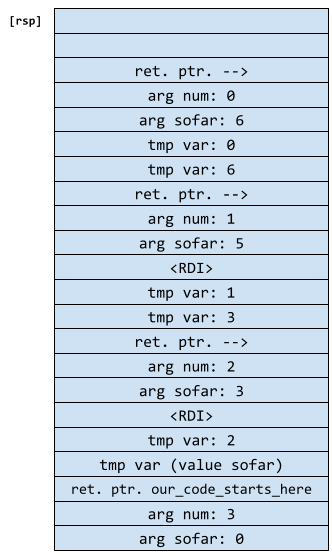
\includegraphics[scale=0.6]{assets/tail_rec_diagram.png}
        \end{center}
    \end{tabular}
\end{center}


\begin{mdframed}
    (Exercise.) What will \code{RAX} be after each return pointer? 

    \begin{mdframed}
        \code{RAX} will be \textbf{6}. There are two ways you can tell: 
        \begin{itemize}
            \item In the code itself, the base case just returns the \code{sofar} argument. Intuitively, this means that this function should return 6 for all subcalls, implying \code{rax} has 6 at every return pointer. 
            \item Additionally, when looking at the generated assembly, notice the \code{move rax, [rsp + 32]} instruction. \code{[rsp + 32]} points to the value \code{sofar}, 6. Pair this with when we look at the instructions after the \code{call} instruction (which is where the program returns to after \code{ret} is executed), notice that there's no additional move instructions to \code{rax}. 
        \end{itemize}
    \end{mdframed}
\end{mdframed}
\textbf{Remark:} There are several things to notice:
\begin{itemize}
    \item there's no use of local variables or arguments following the \code{call} instruction. 
    \item there are no changes to \code{rax} after the \code{call} instruction.
\end{itemize}
These observations means that we can reuse the space that we set up for the function call to perform all operations. In other words, we can use one stack frame's worth of space for the \emph{entire} computation! Basically, we're using more space than we need. 

\subsection{Restructuring the Assembly}
Instead of the \code{call} instruction above, what should we do to replace the instructions so that the new instructions overwrite the current arguments with the new arguments and ``re-use'' the stack frame? 

\bigskip 

We can preemptively add to \code{rsp} to ``undo'' the \code{sub} at the beginning of the function. That is, 
\begin{center}
    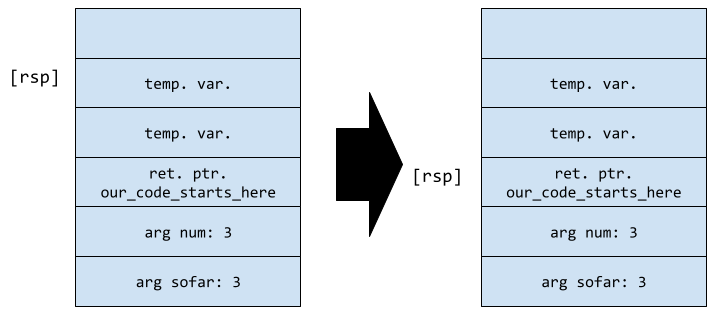
\includegraphics[scale=0.5]{assets/tail_call_2.png}
\end{center}
So, we can write the following assembly:
\begin{verbatim}
    add rsp, 16 
    mov rbx, [rsp - 16]
    mov [rsp + 8], rbx 
    mov [rsp + 16], rax 
    jmp sumrec\end{verbatim}
Notice how we have an \emph{unconditional jump} to \code{sumrec}, as opposed to a \code{call} instruction. This is important, because this effectively means we have a \textbf{loop}!
\begin{center}
    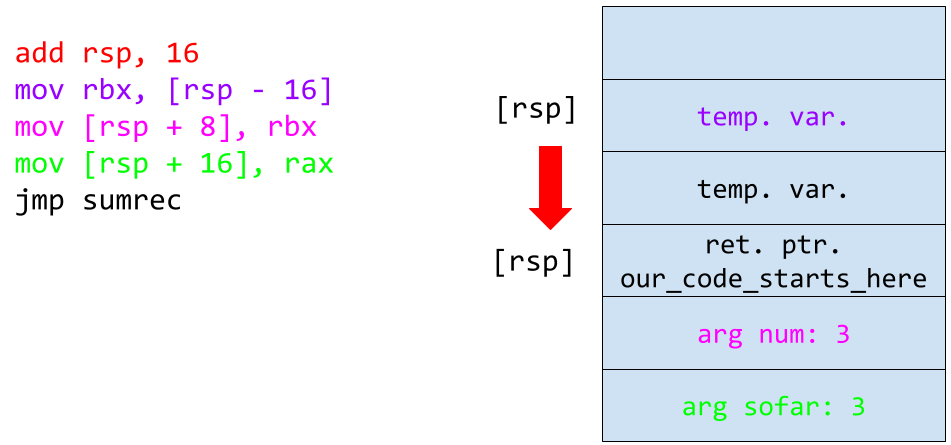
\includegraphics[scale=0.4]{assets/tail_call_3.png}
\end{center}
This process is known as \textbf{proper tail calls}. We effectively re-use the stack from when the ``last thing'' is a function call (what would have been a separate function call with its own stack frame is now a separate ``function call'' re-using the same stack frame from the current ``function call.'').

\subsection{Tail Call Positions}
When is an expression in tail call position? How does the compiler know when it is in tail call position? A few things: 
\begin{itemize}
    \item Anything where we generate instructions that work with the result of a subexpression is not in tail call.  
    \item Essentially, if you work with \code{rax} or store the value after a recursive call to the compile function, that recursive function call cannot be in tail call position. If you don't do anything with it and rely on the answer being in \code{rax} after making the recursive call, then it's in tail position.
\end{itemize}
So, with this in mind: 
\begin{itemize}
    \item \code{Add1}: not in tail call position (adds 1 to \code{rax}). 
    \item \code{Eq}: not in tail call position (needs to store \code{rax} somewhere before compiling the second expression so we can compare them).
    \item \code{Plus}: not in tail call position (needs to store \code{rax} somewhere so we can add to \code{rax} later).
    \item \code{Let}: the value associated with the binding cannot be in tail position, but the body of the \code{let}-expression \emph{can} be in tail position (provided that any preceding calls are in tail position as well).
    \item \code{If}: the conditional expression cannot be in tail position, but the then/else expressions can be in tail position (provided that any preceding calls are in tail position as well).
    \item \code{Block}: only the last expression in a block can be in tail position; the other expressions cannot be in tail position. 
    \item \code{Break}/\code{Loop}: they \emph{generally} cannot be in tail call position (there are special cases, though).
\end{itemize}
In a function call, the arguments cannot be in tail-call position. Note that the body of the expression is where we compile tail call position code or regular code based on whether we're in tail call position. 

\bigskip 

In other words, at the beginning of compilation, we assume that we're in tail call position. As we compile each expression, we might ``lose'' that tail call position. We can never get it back once lost in that subexpression.